\documentclass[conference]{IEEEtran}

% ---- Packages ----
\usepackage{iftex}
\ifPDFTeX
  \usepackage[utf8]{inputenc}
\fi
\usepackage[T1]{fontenc}
\usepackage{amsmath,amssymb,amsthm}
\usepackage{algorithm}
\usepackage{booktabs}
\usepackage{array}
\usepackage{calc}
\usepackage{adjustbox}
\usepackage{graphicx}
\usepackage{tikz}
\usepackage{pgfplots}
\pgfplotsset{compat=1.18}
\usepackage{listings}
\usepackage[varqu]{zi4}
\usepackage{xcolor}
\usepackage{textcomp}
\usepackage{balance}
\usepackage{url}
\usepackage{cite}
\usepackage{hyperref}
\hypersetup{hidelinks}

% pandoc helpers
\providecommand{\tightlist}{\setlength{\itemsep}{0pt}\setlength{\parskip}{0pt}}

% ---- Float placement: the paper has many double-column floats, so let pages carry more of them ----
\setcounter{topnumber}{3}
\setcounter{dbltopnumber}{3}
\setcounter{totalnumber}{6}
\renewcommand{\topfraction}{0.95}
\renewcommand{\dbltopfraction}{0.95}
\renewcommand{\textfraction}{0.05}
\renewcommand{\floatpagefraction}{0.8}
\renewcommand{\dblfloatpagefraction}{0.8}
\makeatletter
\setlength{\@fptop}{0pt}
\setlength{\@fpsep}{14pt}
\setlength{\@fpbot}{0pt plus 1fil}
\setlength{\@dblfptop}{0pt}
\setlength{\@dblfpsep}{14pt}
\setlength{\@dblfpbot}{0pt plus 1fil}
\makeatother

% ---- Pseudocode and code listing style ----
\lstdefinestyle{pseudo}{
  basicstyle=\ttfamily\scriptsize,
  keywordstyle=\bfseries,
  showstringspaces=false,
  breaklines=true,
  breakatwhitespace=true,
  frame=single,
  framesep=2pt,
  xleftmargin=4pt,
  xrightmargin=4pt,
  aboveskip=6pt,
  belowskip=4pt,
  columns=fullflexible,
  morekeywords={ALGORITHM,LOOP,EXIT,RETURN,FOR,EACH,IN,IF,WHERE,EXISTS}
}

% Columns end where their text ends; stretching them left gaps inside columns next to wide floats.
\raggedbottom

\begin{document}
\title{Ancestor-Partitioned Index Projections for Authorized Pagination in Hierarchical Role-Based Access Control}
\author{\IEEEauthorblockN{Ross Slaney}}
\maketitle

\begin{abstract}
In scoped hierarchical role-based access control, a role assigned to a principal at a node of a resource hierarchy applies at that node and at all of its descendants, as in Azure role-based access control. The SHRBAC model enforces these semantics inside an application's relational database with an inline table-valued function that composes with application queries, and a single access decision examines a bounded number of ancestors and principals. Ordered pagination over authorized rows does not inherit this bound. Evaluating the function on rows read in index order examines every row that precedes the last authorized row of the page, and this number grows as the caller's authorized rows become sparse in the order or occur late in it. We introduce ancestor-partitioned index projections, which store, for each index of a protected table, one entry per row and active ancestor, keyed by the ancestor, the index key and the row key. The rows below any node then occupy a contiguous range in index order, and a page of \(P\) rows is computed by merging at most \(P\) entries from the range of each of the caller's minimal granted scopes and verifying the selected rows with the original function. We prove the method sound for any state of the projections and complete when they are consistent with the base tables, and we bound the cost of a page by a function of the page size, the depth of the hierarchy and the caller's grants and scopes that does not depend on the table size or on the fraction of rows the caller may access. With 1,000,000 rows on SQL Server 2022 and PostgreSQL 16, the rows read for a first page fall from 368,410 and 184,205 to 100 and 80 for a caller with access to 100 rows, and from 1,960,040 and 980,020 to 100 and 80 for a caller whose rows occur at the end of the order. Callers with many individual grants remain the most expensive case.
\end{abstract}

\section{Introduction}\label{sec-1}

Role-based access control assigns permissions to roles and roles to principals \cite{ref1}, \cite{ref2}. Many deployed systems also scope each assignment to a node of a resource hierarchy, so that the permissions conferred by a role apply at that node and at every node below it. Azure role-based access control (Azure RBAC) follows this scoped hierarchical model \cite{ref3}. In Azure RBAC, a role assignment consists of a security principal, a role definition and a scope. Security principals are users, groups, service principals and managed identities; a role definition is a collection of permissions; and a scope is a management group, a subscription, a resource group or an individual resource \cite{ref3}, \cite{ref4}. Scopes form a parent--child hierarchy in which lower levels inherit role permissions from higher levels \cite{ref5}, and a principal's effective permissions are the sum of its role assignments \cite{ref3}. A role assigned to a group at a resource group thus authorizes the members of the group on every resource in that resource group.

Applications that manage their own resources organize them in the same way. A retailer's products belong to stores, regions and chains, and the items of a multi-tenant software product belong to projects, workspaces and organizations; responsibility is assigned at one level of such a hierarchy. Authorization services for application developers provide these semantics. WorkOS arranges an application's resources in a hierarchy down which permissions flow \cite{ref6}, OpenFGA allows a relation on a parent object, such as the editors of a folder, to apply to the objects it contains \cite{ref7}, and Zanzibar expresses inheritance from parent objects through userset rewrite rules \cite{ref8}.

SHRBAC (Scoped Hierarchical Role-Based Access Control) \cite{ref9} applies this model to resources defined by an application and enforces it inside the application's relational database. Resources, principals, roles and grants are stored as tables, and a grant assigns a role to a principal at a resource for an optional validity interval. The access decision is an inline table-valued function that walks from a row's resource toward the root of the hierarchy and joins, at each ancestor, the active grants of the caller's principals. Because the optimizer expands the function into the calling query, an application can add it as a predicate to its own queries, and authorization then composes with the query's filters, sort order and cursor pagination in a single statement. The authorization concepts are those of scoped hierarchical RBAC. The earlier work \cite{ref9} contributes their enforcement inside the database over application-defined resources, with proofs that the predicate is sound and complete and a bound on its cost. A single decision examines at most \(D\) ancestors for each of \(M\) effective principals, and on a hierarchy of depth 9 with 1.5 million resources, point decisions took under 1.5 ms (median).

The cost of a single decision does not determine the cost of enumeration. To return the first \(P\) authorized rows of a query in the order of an index, the predicate is evaluated on rows in index order until \(P\) of them are authorized, so the work per page is proportional to the number of rows that precede the \(P\)-th authorized row. That number depends on where the caller's authorized rows occur in the order. For a caller with access to a fraction \(\sigma\) of the rows, distributed uniformly, about \(P/\sigma\) rows are examined per page; for a caller whose authorized rows are the last \(V\) rows of the order, the first page examines \(N - V + P\) rows. The complexity analysis of \cite{ref9} states this dependence, and its evaluation concentrated on workloads in which authorized rows are dense in the order. In a table of 1,000,000 products on PostgreSQL 16, a first page of 20 rows examines 184,205 rows for a store manager with access to 100 products and 980,020 rows for a caller whose 20,000 products occur at the end of the price order (Section~\ref{sec-7}). Enumeration is also the operation that external authorization services restrict. OpenFGA's ListObjects call returns at most 1,000 results within 3 seconds by default \cite{ref10}, and SpiceDB's documentation recommends its LookupResources call when a user can access fewer than about 10,000 resources \cite{ref11}.

Under hierarchical inheritance, the rows a caller may access form the union of the subtrees below the scopes at which the caller holds a qualifying grant. Predicate evaluation in index order is expensive for sparse callers because the index orders all rows of the table and interleaves the rows of any one subtree with all others. The method presented here maintains, for each index, the rows of every subtree in index order. An ancestor-partitioned index projection stores one entry for every row and every active ancestor of the row's resource, keyed by the ancestor, the index key and the row key. The rows below any scope form one contiguous range of the projection, ordered by the index key, and the first \(P\) authorized rows after a cursor are found among the first \(P\) entries after the cursor in the ranges of the caller's minimal granted scopes. A page therefore requires \(k\) bounded range reads and a \(k\)-way merge, where \(k\) is the number of such scopes, followed by verification of each selected row with the original access function. The projections are derived data. They are updated in the transaction of each write and can be rebuilt from the base tables, and they do not determine access, since a row is returned only if the access function admits it when the statement executes.

The contributions of this paper are the following.

\begin{itemize}
\tightlist
\item
  An analysis of authorized ordered pagination under scoped hierarchical RBAC. With predicate evaluation in index order, the rows examined per page are the rows that precede the \(P\)-th authorized row; with enumeration through an unordered ancestor closure, they are the caller's authorized rows. Both quantities are determined by the caller's grants, and each is proportional to the table size for some callers (Section~\ref{sec-3}).
\item
  Ancestor-partitioned index projections, minimal granted scopes computed within the database, and a pagination algorithm that combines an ordered scan, a merge of projection ranges, and verification by the access function (Section~\ref{sec-4}).
\item
  Proofs that the algorithm is sound for any state of the projections and complete for consistent projections, a per-page bound that is independent of the table size and of the caller's selectivity, and bounds on projection storage and maintenance (Section~\ref{sec-5}).
\item
  An implementation for SQL Server and PostgreSQL in which projections are derived from the application's index declarations and maintained in the writing transaction (Section~\ref{sec-6}), and an evaluation with 1,000,000 rows against predicate evaluation and closure enumeration for dense, sparse, late-ordered and many-grant callers, including storage and update costs (Section~\ref{sec-7}).
\end{itemize}

Section~\ref{sec-8} reviews related work, and Section~\ref{sec-9} discusses limitations.

\section{Background}\label{sec-2}

\subsection{Scoped Hierarchical Role-Based Access Control}\label{sec-2-1}

RBAC96 and the NIST RBAC standard assign permissions to roles and roles to users, with an optional hierarchy among roles \cite{ref1}, \cite{ref2}; the resources to which permissions refer are not structured. Scoped hierarchical models add a hierarchy of resources or organizational units and qualify each assignment with a node of that hierarchy, as in ROBAC \cite{ref12} and in RBAC with resource hierarchies \cite{ref13}. The relationship of SHRBAC to these models is discussed in \cite{ref9}.

Azure RBAC is an authorization system built on Azure Resource Manager that provides access management for Azure resources \cite{ref3}, and it serves here as the reference example of scoped hierarchical RBAC. A role definition lists the control-plane operations (Actions) and data-plane operations (DataActions) that a role permits, together with operations excluded from them (NotActions and NotDataActions). The effective control-plane permissions of a role are its Actions less its NotActions, and an exclusion is not a denial, since another role assignment may grant the excluded operation \cite{ref14}. Scopes are specified at four levels, namely management groups, subscriptions, resource groups and resources \cite{ref5}. Management groups form a tree of up to six levels below the root, and each management group and subscription can have only one parent \cite{ref15}. Role assignments to groups are transitive, so a member of a group that is itself a member of a group with a role assignment holds the permissions of that assignment \cite{ref3}. Azure also maintains deny assignments, which block actions even when a role assignment grants them and which, in generally available scenarios, are created and managed by Azure rather than by customers \cite{ref16}. Role assignments may carry attribute-based conditions \cite{ref4}, and assignments with start and end dates are available through Privileged Identity Management \cite{ref17}. To decide a request, Azure Resource Manager retrieves the role assignments and deny assignments that apply to the target resource, blocks the request if a deny assignment applies, determines the roles that the caller and its groups hold for the resource, checks whether the requested action is among their permissions, and evaluates any conditions \cite{ref3}.

Table~\ref{tab:1} compares Azure RBAC with SHRBAC. The two share the principal--role--permission--scope structure, the inheritance of assignments by descendant scopes, and the additive combination of assignments. They differ in the hierarchy, which in SHRBAC is an application-defined tree of resources of arbitrary types; in group semantics, which in SHRBAC are not recursive; in the absence from SHRBAC of negative authorizations and attribute conditions; and in where authorization is enforced, which in Azure RBAC is the evaluation of individual requests by the resource manager and in SHRBAC is a predicate evaluated by the application's database within its queries.

\begin{table*}[!tp]
\centering
\caption{Azure RBAC and SHRBAC.}
\label{tab:1}
\scriptsize
\begin{adjustbox}{max width=\textwidth}
\begin{tabular}{@{}
  >{\raggedright\arraybackslash}p{(\textwidth - 4\tabcolsep) * \real{0.1600}}
  >{\raggedright\arraybackslash}p{(\textwidth - 4\tabcolsep) * \real{0.4200}}
  >{\raggedright\arraybackslash}p{(\textwidth - 4\tabcolsep) * \real{0.4200}}@{}}
\toprule\noalign{}
\begin{minipage}[b]{\linewidth}\raggedright
Concept
\end{minipage} & \begin{minipage}[b]{\linewidth}\raggedright
Azure RBAC
\end{minipage} & \begin{minipage}[b]{\linewidth}\raggedright
SHRBAC
\end{minipage} \\
\midrule\noalign{}
Principals & users, groups, service principals, managed identities & users, groups, service accounts, agents \\
Role & role definition: Actions and DataActions, less NotActions and NotDataActions & set of permissions \\
Scope hierarchy & management groups (up to six levels below the root), subscriptions, resource groups, resources; one parent per node & application-defined tree of typed resources of depth at most \(D\); one parent per node \\
Assignment & role assignment: principal, role definition, scope & grant: principal, role, resource, validity interval \\
Inheritance & lower levels inherit role permissions from higher levels & a grant applies at its resource and at every descendant reached through active resources \\
Multiple assignments & additive & additive \\
Group membership & transitive & one level; groups do not contain groups \\
Negative authorization & deny assignments, created by Azure & none \\
Other conditions & attribute conditions; start and end dates through Privileged Identity Management & validity interval of each grant \\
Enforcement & evaluated for each request by Azure Resource Manager or integrated data-plane services & evaluated by the application's database as a predicate within each query \\
\bottomrule
\end{tabular}
\end{adjustbox}
\end{table*}

\subsection{The SHRBAC Model}\label{sec-2-2}

We restate the definitions of \cite{ref9} used in this paper, with two conditions that its implementation applies: an inactive resource interrupts inheritance, and a permission may be restricted to one resource type.

Resources form a rooted tree of depth at most \(D\), and each resource may be marked inactive. For a resource \(r\), \(\mathrm{anc}(r)\) is the sequence \(r, \mathrm{parent}(r), \mathrm{parent}(\mathrm{parent}(r)), \ldots\) up to the root, which includes \(r\). The active ancestor path \(\mathrm{anc}^{+}(r)\) is the longest prefix of \(\mathrm{anc}(r)\) whose resources are all active; it is empty when \(r\) is inactive.

Principals are users, groups, service accounts and agents. For a principal \(p\), \(\mathrm{resolve}(p)\) contains \(p\) and, if \(p\) is a user, the active groups of which \(p\) is a member; groups do not contain groups. We write \(M = |\mathrm{resolve}(p)|\). A role is a set of permissions, \(\mathrm{perms}(\mathit{role})\), and a permission may be restricted to one resource type. A grant \((p, \mathit{role}, x, t_1, t_2)\) assigns a role to principal \(p\) at resource \(x\) for the interval \([t_1, t_2]\), either bound of which may be absent; it is active at time \(t\) if \(t\) lies in the interval.

\textbf{Definition 1 (Access decision).} For a principal \(p\), permission \(\mathit{perm}\), resource \(r\) and time \(t\), \(\mathrm{allowed}(p, \mathit{perm}, r, t)\) holds if and only if there exist \(p' \in \mathrm{resolve}(p)\), a resource \(x \in \mathrm{anc}^{+}(r)\) and a grant \((p', \mathit{role}, x, t_1, t_2)\) active at \(t\) with \(\mathit{perm} \in \mathrm{perms}(\mathit{role})\), and, if \(\mathit{perm}\) is restricted to a resource type, \(r\) has that type.

A protected table \(T\) is an application table whose rows carry a column ResourceId that names a resource; \(\mathrm{res}(r)\) denotes the resource of row \(r\). A row \(r\) is authorized for \(p\) and \(\mathit{perm}\) at \(t\) if \(\mathrm{allowed}(p, \mathit{perm}, \mathrm{res}(r), t)\) holds.

\subsection{Database-Native Enforcement}\label{sec-2-3}

The implementation of \cite{ref9} expresses Definition 1 as an inline table-valued function, \texttt{fn\_IsResourceAccessible}, referred to below as the access function, whose arguments are a resource identifier, the caller's principal identifiers and a permission identifier. A recursive common table expression walks from the resource toward the root for at most \(D\) steps, and each step is joined with the active grants of the given principals whose roles carry the permission. Because the function is inline, the optimizer expands its body into the calling query, and an application restricts a query to authorized rows with the condition \texttt{EXISTS\ (SELECT\ 1\ FROM\ fn\_IsResourceAccessible(T.ResourceId,\ ...))}. The function is sound and complete with respect to Definition 1 for hierarchies within the depth bound \cite{ref9}, and one evaluation costs \(O(D \cdot M \cdot G_{\max})\) index lookups, where \(G_{\max}\) is the largest number of active grants that one principal holds at one resource. With cursor pagination on an indexed sort key, a page of \(P\) rows costs \(O(P \cdot D \cdot M \cdot G_{\max})\) when nearly all rows are authorized, \(O(P/\sigma \cdot D \cdot M \cdot G_{\max})\) when a fraction \(\sigma\) of the rows is authorized, and \(O(N \cdot D \cdot M \cdot G_{\max})\) when no row is. The same function serves as the point check for a single resource. It is used unchanged in the first and last phases of the algorithm in Section~\ref{sec-4-4}.

\textbf{Notation.} \(N\) is the number of rows of the paged table, \(P\) the page size, \(D\) the depth bound of the hierarchy, and \(L(r) = |\mathrm{anc}^{+}(\mathrm{res}(r))| \le D + 1\) the number of active ancestors of a row's resource. For a given caller and permission, \(V\) is the number of authorized rows, \(\sigma = V/N\), \(G\) the number of active grants held by the caller's principals whose roles carry the permission, and \(k\) the number of minimal granted scopes (Section~\ref{sec-4-3}). \(R\) is the number of rows examined by predicate evaluation in index order (Section~\ref{sec-3-2}), and \(I\) the number of projected orderings of a table (Section~\ref{sec-4-2}). As in \cite{ref9}, an index seek counts as one operation; with B-tree indexes, a seek costs \(O(\log N)\) page accesses.

\section{Authorized Ordered Pagination}\label{sec-3}

\subsection{Problem Definition}\label{sec-3-1}

Let \(T\) be a protected table with primary key \(\kappa\). An ordering \(K = (c_1, \ldots, c_m, \kappa)\) is a sequence of columns of \(T\) that ends with the primary key and therefore orders the rows of \(T\) totally; we write \(r <_K s\), and \(K(r)\) for the values of \(K\) in row \(r\). A paged query \(Q = (T, \varphi, K)\) restricts \(T\) by an application-defined predicate \(\varphi\) and orders it by \(K\), ascending or descending. A cursor \(u\) is either empty or a tuple of values of \(K\).

\textbf{Definition 2 (Authorized page).} For a caller \(p\), permission \(\mathit{perm}\), time \(t\), cursor \(u\) and page size \(P\), the authorized page of \(Q\) is the sequence of the first \(P\) rows \(r\) of \(T\) in \(K\) order such that \(K(r)\) follows \(u\), \(\varphi(r)\) holds, and \(r\) is authorized for \(p\) and \(\mathit{perm}\) at \(t\). If fewer than \(P\) rows qualify, the page contains all of them.

Each page is returned with a cursor that marks its end in \(K\) order, and requesting pages until one is returned without a cursor enumerates the authorized rows of \(Q\) in \(K\) order. This is keyset pagination, whose cost does not depend on the number of preceding pages \cite{ref9}.

The setting places several conditions on any method. The application owns \(T\) and its schema, so a method may add only the ResourceId column and an index on it, and any other structure resides in separate tables. Authorization state resides in the same database, and a statement receives only the caller's principal identifiers and the permission identifier as authorization inputs. Sets derived from the caller's grants, such as the scopes at which the caller holds grants, are computed within the statement, since their size is not bounded. Derived structures are updated in the transaction of each write that changes their inputs, and every returned row satisfies Definition 1 when the statement executes. The objective is a cost per page that is bounded independently of \(N\) and of the caller's selectivity.

\subsection{Predicate Evaluation in Index Order}\label{sec-3-2}

The method of \cite{ref9} computes a page by reading the rows of \(Q\) that follow \(u\) in \(K\) order, through an index on \(K\), and evaluating the access function on each row until \(P\) rows are authorized. Let \(R(u)\) be the number of rows of \(Q\) that follow \(u\), up to and including the \(P\)-th authorized row, or all rows of \(Q\) after \(u\) if fewer than \(P\) are authorized. The page costs \(\Theta(R(u))\) row accesses and \(R(u)\) evaluations of the access function, each \(O(D \cdot M \cdot G_{\max})\).

\(R(u)\) is determined by the positions of the caller's authorized rows in \(K\) order. If the caller is authorized for a fraction \(\sigma\) of the rows of \(Q\) and these rows are distributed uniformly in \(K\) order, \(R(u)\) is about \(P/\sigma\). If the caller's \(V\) authorized rows are the last \(V\) rows of \(Q\), the first page has \(R = N - V + P\). Fig.~\ref{fig:1} shows both cases for the workload of Section~\ref{sec-7}, where \(R = 184{,}205\) for a caller with 100 authorized rows distributed through the order and \(R = 980{,}020\) for a caller with 20,000 authorized rows at its end. An index on the inputs of the access function, such as ResourceId, does not change \(R\), which depends on which rows are authorized rather than on the cost of each decision.

\begin{figure*}[!tp]
\centering
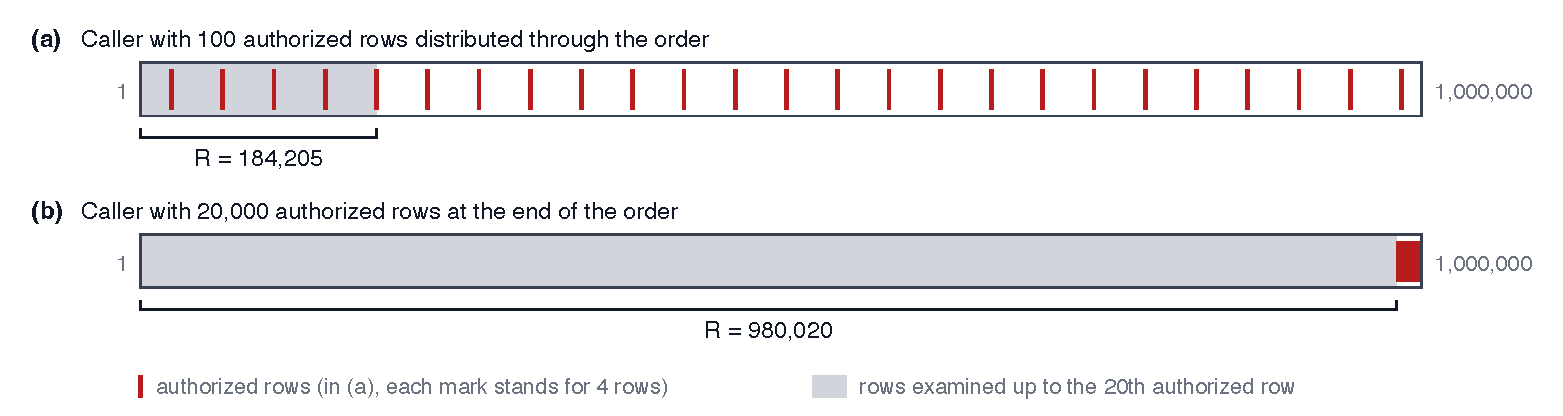
\includegraphics[width=\textwidth]{figures/sparse-problem.pdf}
\caption{Rows examined by predicate evaluation for a first page of 20 rows in (Price, Id) order, in a table of 1,000,000 rows on PostgreSQL 16. (a) A caller with 100 authorized rows distributed through the order. (b) A caller with 20,000 authorized rows at the end of the order.}
\label{fig:1}
\end{figure*}


\subsection{Enumeration Through an Ancestor Closure}\label{sec-3-3}

The dependence on position can be removed by enumerating the caller's rows directly. The ancestor closure of \(T\) is the set of pairs \((x, r)\) with \(r \in T\) and \(x \in \mathrm{anc}^{+}(\mathrm{res}(r))\), indexed by \(x\). A caller's authorized rows are the rows paired with the resources at which the caller holds a qualifying grant, so they can be read from the closure without examining unauthorized rows. The closure does not order them by \(K\), however. Returning the first \(P\) in \(K\) order requires reading all of the caller's rows that satisfy \(\varphi\) and follow \(u\) and selecting the first \(P\), which costs \(\Theta(V)\) row accesses for the first page. This cost does not depend on position, but it is proportional to the number of rows the caller may access.

A method that runs both access paths in rounds with growing budgets, and takes the page from whichever path completes first, reads \(O(\min(R, V) + P)\) rows. This bound is still proportional to the table size for some callers. For the caller whose 20,000 rows occur at the end of the order, \(V = 0.02N\) and \(R = N - V + P\), so both terms grow linearly with \(N\) when the caller's share of the table is fixed.

Selecting one path in advance requires knowing \(R\) and \(V\), which are functions of the caller's grants rather than properties of any column of \(T\). The column statistics from which a cost-based optimizer selects a plan are the same for every caller. A bound that depends on neither \(R\) nor \(V\) is obtained when the rows below each scope can be read in \(K\) order, which is the structure defined in Section~\ref{sec-4}.

\section{Ancestor-Partitioned Index Projections}\label{sec-4}

\subsection{Definition}\label{sec-4-1}

\textbf{Definition 3 (Projection).} For a protected table \(T\) and an ordering \(K\), the ancestor-partitioned index projection of \(T\) on \(K\) is the relation

\[\Pi_K(T) = \{\, (x, K(r)) : r \in T,\ x \in \mathrm{anc}^{+}(\mathrm{res}(r)) \,\}.\]

It is stored in a separate table with primary key \((x, c_1, \ldots, c_m, \kappa)\) and a secondary index on \(\kappa\). A stored projection is consistent with \(T\) and the resource tables if it contains exactly these entries.

The membership condition is the reachability condition of Definition 1, under which a grant at resource \(x\) can authorize row \(r\) only if \(x \in \mathrm{anc}^{+}(\mathrm{res}(r))\). The entries whose first component is \(x\), read in primary-key order, are the rows below \(x\) in \(K\) order. Each row has \(L(r) \le D + 1\) entries in each projection, and a row whose resource is inactive has none.

Fig.~\ref{fig:2} shows a projection on \((\mathrm{Price}, \mathrm{Id})\) for four products whose resources are two stores of one region. The range of each store lists that store's products in price order, the range of region R1 lists all four products in price order, and the ranges of the chain, the division and the root repeat the same four entries.

\begin{figure*}[!tp]
\centering
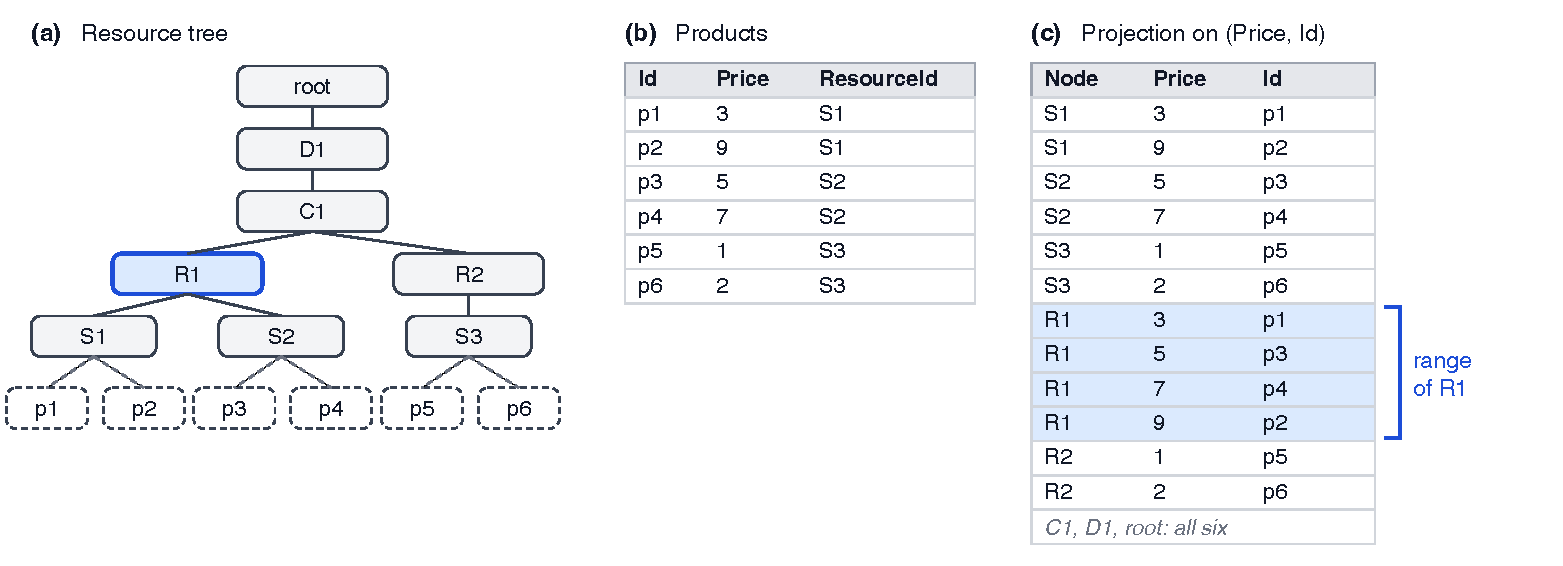
\includegraphics[width=\textwidth]{figures/storage.pdf}
\caption{Example of a projection on (Price, Id). (a) Resource tree; the dashed boxes are rows of the Products table, whose ResourceId values name stores S1 and S2. (b) The Products table. (c) The projection, with one entry for each product and each active ancestor of its resource, ordered by (Price, Id) within each node. The highlighted entries form the range of region R1, and the entries under C1, D1 and the root repeat them.}
\label{fig:2}
\end{figure*}


\subsection{Projected Orderings}\label{sec-4-2}

The orderings for which projections are maintained are derived from the indexes of \(T\). The primary key defines one projected ordering. Every other index defines the ordering that consists of its columns followed by the primary key; an index that already ends with the primary key defines the same ordering as the index without it, and uniqueness, filters, descending columns and included columns are disregarded. Because a B-tree can be read in either direction, one projection serves ascending and descending pages. Two classes of index serve lookups rather than orderings and are not projected: indexes that contain ResourceId, and indexes whose columns are exactly the columns of a foreign key. An index with a column that cannot be part of a projection key, such as a nullable column, is not projected either.

A paged query uses \(\Pi_K\) if and only if its ordering, with the primary key appended, equals \(K\) column by column, so an ordering by name and then city requires an index on (name, city). An ordering without a projection is evaluated by the scan phase of the algorithm alone, at a cost of \(O(R)\) rows.

\subsection{Minimal Granted Scopes}\label{sec-4-3}

\textbf{Definition 4 (Minimal granted scopes).} For a caller \(p\), permission \(\mathit{perm}\) and time \(t\), a resource \(x\) is a qualifying scope if it is active and some \(p' \in \mathrm{resolve}(p)\) holds a grant at \(x\) that is active at \(t\) and whose role carries \(\mathit{perm}\). \(S(p, \mathit{perm}, t)\) is the set of qualifying scopes \(x\) such that no resource of \(\mathrm{anc}^{+}(x)\) other than \(x\) is a qualifying scope. We write \(k = |S(p, \mathit{perm}, t)|\).

A grant at a resource below another qualifying scope contributes no additional rows, since every row below it is also below the higher scope. \(S\) is computed within the statement by a table-valued function, referred to below as the scope function, whose only authorization inputs are the principal identifiers and the permission identifier. It applies the same principal, role, validity and activity conditions as the access function and removes every qualifying scope that has a qualifying scope among its active ancestors.

\subsection{Pagination Algorithm}\label{sec-4-4}

Algorithm~\ref{alg:1} computes an authorized page in rounds with a budget \(b\) that starts at \(P\).

\begin{algorithm}[!t]
\caption{Authorized pagination over ancestor-partitioned projections.}
\label{alg:1}
\begin{lstlisting}[style=pseudo]
ALGORITHM AuthorizedPage(Q, p, perm, u, P)
  // Q = (T, phi, K); u is the cursor
  pr <- resolve(p); q <- lookup(perm); b <- P
  LOOP
    // Scan phase
    rows <- first b rows of Q after u in K order,
            each with a(r) = AccessFn(res(r), pr, q)
    A <- those rows with a(r) true
    IF |A| >= P: sel <- first P rows of A; EXIT LOOP
    IF |rows| < b: sel <- A; EXIT LOOP
    // Merge phase
    IF a projection Pi_K exists:
      FOR EACH x IN ScopeFn(pr, q):
        E[x] <- first b entries of Pi_K under x
                after u whose row satisfies phi
      sel <- first P entries of the union of
             all E[x], in K order
      EXIT LOOP
    b <- 4 * b
  // Verification
  page <- the rows of Q with keys in sel and
          AccessFn(res(r), pr, q), in K order
  cursor <- none if the scan or the merge ran
            out of rows, else K(last entry of sel)
  RETURN (page, cursor)
\end{lstlisting}
\end{algorithm}

The scan phase reads the next \(b\) rows of \(Q\) in \(K\) order after \(u\) and evaluates the access function on each row within the same statement. If at least \(P\) of them are authorized, the first \(P\) form the page. If fewer than \(b\) rows remain, the query is exhausted and its remaining authorized rows form the last page. A caller who is authorized for most rows obtains the page in this phase, as does a query whose filter already restricts \(T\) to one of the caller's scopes, for example a single store.

The merge phase runs when the scan phase does not complete the page and a projection exists for \(K\). For each \(x \in S\), it reads the first \(b\) entries of \(\Pi_K\) with first component \(x\) that follow \(u\) and whose row satisfies \(\varphi\), and it merges these ranges in \(K\) order, retaining the first \(P\) entries. Because \(b \ge P\), the merge phase completes the page in the round in which it runs: either \(P\) entries are returned, or every range is exhausted and the returned entries are the remaining rows below the caller's scopes. The budget grows to \(4b\) only for orderings without a projection, for which the scan phase is repeated with the larger budget.

Verification loads the selected rows of \(Q\) by key, evaluates the access function on each row, and returns the rows in \(K\) order. The cursor holds the values of \(K\) for the last row selected by the scan or merge phase, so that rows removed by verification are not selected again by the next page; it is empty when the scan phase reached the end of \(Q\) or every range was exhausted. For an ordering with a projection, a page therefore issues at most five statements: two that resolve the principals and the permission, the scan, the merge, and the verification.

Fig.~\ref{fig:3} traces a page for a caller with a grant on one store in the workload of Section~\ref{sec-7}. The scan phase reads 20 rows, none of which are authorized, the merge phase reads the first 20 entries of the store's range together with the corresponding rows, and verification reads the 20 selected rows.

\begin{figure*}[!tp]
\centering
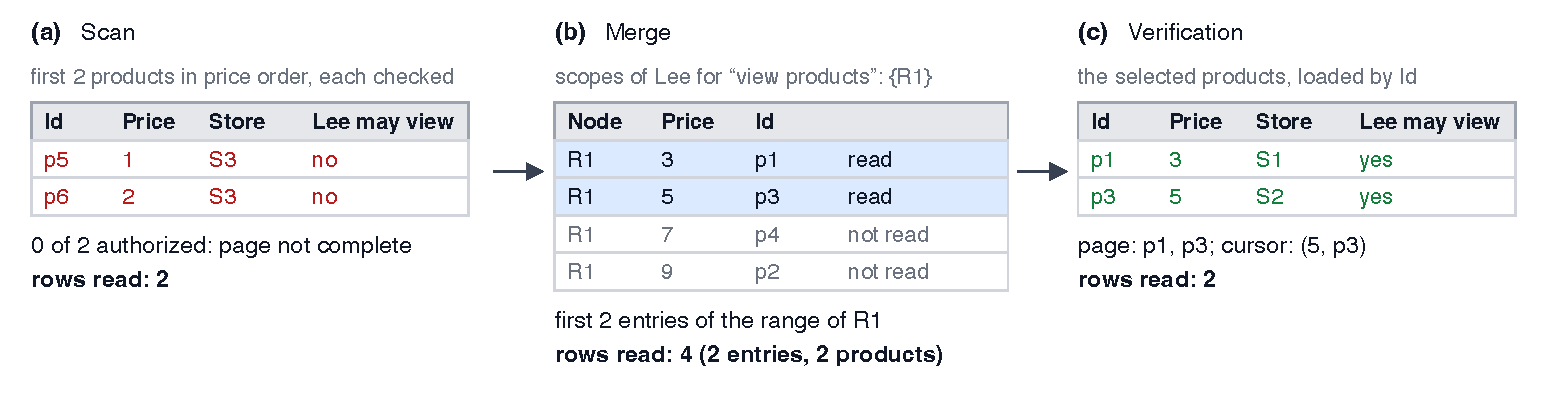
\includegraphics[width=\textwidth]{figures/retrieval.pdf}
\caption{Computation of a first page for a caller with a grant on one of the 10,000 stores of Section~\ref{sec-7}. (a) None of the first 20 rows in (Price, Id) order is authorized. (b) The scope function returns the caller's store S7, and the merge phase reads the first 20 entries of its range together with the corresponding rows. (c) Verification evaluates the access function on the 20 selected rows. The three phases read 80 rows on PostgreSQL 16.}
\label{fig:3}
\end{figure*}


\subsection{Maintenance}\label{sec-4-5}

Projections are updated in the transaction of every write that changes their inputs. Inserting or deleting a row, or changing its ResourceId or a projected column, deletes the row's entries through the index on \(\kappa\) and inserts entries for \(\mathrm{anc}^{+}(\mathrm{res}(r))\). Moving a resource to a new parent, or changing whether it is active, changes \(\mathrm{anc}^{+}\) for every row below it, and the entries of those rows are recomputed by walking the resource's subtree. Every committed write is reflected in every projection, and a write that is rolled back leaves no entries. Writes that bypass this mechanism, such as bulk loads, require a rebuild that recomputes each projection from \(T\) and the resource tables; the same procedure fills the projection of a newly created index. Fig.~\ref{fig:4} shows the entries written by an insertion and by a move.

\begin{figure*}[!tp]
\centering
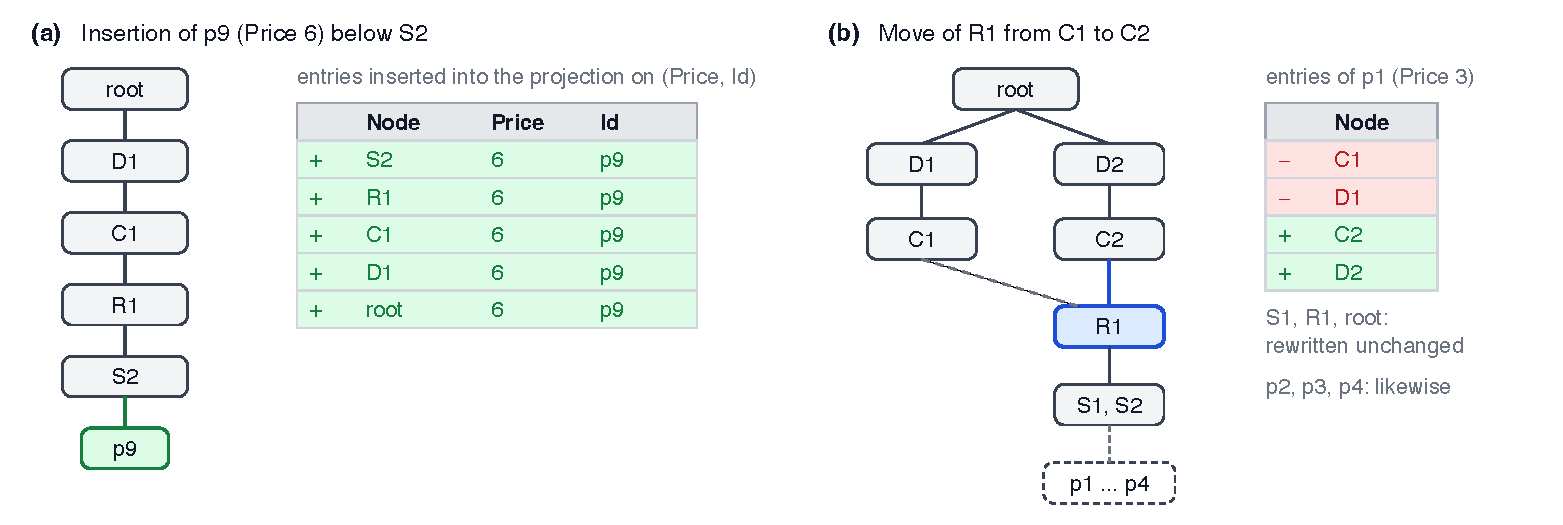
\includegraphics[width=\textwidth]{figures/maintenance.pdf}
\caption{Projection maintenance in the example of Fig.~\ref{fig:2}. (a) Inserting product p9 with price 6 below store S2 inserts one entry for each active ancestor of S2 into every projection. (b) Moving region R1 from chain C1 to chain C2 deletes and reinserts the entries of every row below R1; for p1, the entries under C1 and D1 are replaced by entries under C2 and D2. Both updates run in the transaction of the write.}
\label{fig:4}
\end{figure*}


\section{Correctness and Complexity}\label{sec-5}

\subsection{Soundness}\label{sec-5-1}

\textbf{Theorem 1 (Soundness).} For any contents of the projections, every row returned by Algorithm~\ref{alg:1} is authorized for the caller and the permission at the time verification executes.

\emph{Proof.} Rows are returned only by verification, which evaluates the access function on each selected row. By Theorem 1 of \cite{ref9}, the access function returns a result only for rows that satisfy Definition 1. The scan and merge phases determine which rows are selected, and no selected row is returned without passing verification. \(\square\)

Soundness therefore does not depend on the projections, which affect which rows are found but not which rows are allowed.

\subsection{Completeness}\label{sec-5-2}

\textbf{Lemma 1 (Projection membership).} If \(\Pi_K\) is consistent, then for every row \(r\) and resource \(x\), \(\Pi_K\) contains an entry for \(r\) under \(x\) if and only if \(x \in \mathrm{anc}^{+}(\mathrm{res}(r))\), which is the condition that Definition 1 places on the resource of a grant that authorizes \(r\).

\emph{Proof.} Immediate from Definition 3 and the definition of consistency. \(\square\)

\textbf{Lemma 2 (Disjoint cover).} Let \(\mathit{perm}\) be unrestricted or restricted to the type of \(\mathrm{res}(r)\). Then \(r\) is authorized for \(p\) and \(\mathit{perm}\) at \(t\) if and only if some element of \(S(p, \mathit{perm}, t)\) lies in \(\mathrm{anc}^{+}(\mathrm{res}(r))\), and at most one element of \(S(p, \mathit{perm}, t)\) does.

\emph{Proof.} If \(r\) is authorized, a qualifying scope \(y\) lies in \(\mathrm{anc}^{+}(\mathrm{res}(r))\). Let \(y^{*}\) be the qualifying scope on this path that is closest to the root. Since \(\mathrm{anc}^{+}(y^{*})\) is the part of the path from \(y^{*}\) upward, it contains no other qualifying scope, so \(y^{*} \in S\). Conversely, an element of \(S\) on the path is a qualifying scope, so \(r\) is authorized. If two elements of \(S\) lay on the same path, the higher one would belong to the active ancestor path of the lower one, which contradicts the minimality of the lower one. \(\square\)

\textbf{Theorem 2 (Completeness).} Suppose \(\Pi_K\) is consistent and \(\mathit{perm}\) is unrestricted or restricted to a type shared by the resources of all rows of \(T\). Then Algorithm~\ref{alg:1} returns the authorized page of Definition 2, and the cursor it returns continues the enumeration without omitting or repeating an authorized row.

\emph{Proof.} If the scan phase completes the page, it has read the rows of \(Q\) after \(u\) in \(K\) order and evaluated the access function on each, which is sound and complete \cite{ref9}; its selection consists of the first \(P\) authorized rows, or all of them if the query is exhausted. Otherwise the merge phase runs. By Lemmas 1 and 2, the authorized rows after \(u\) that satisfy \(\varphi\) are the disjoint union, over \(x \in S\), of the rows with an entry under \(x\) after \(u\) that satisfy \(\varphi\). Each range lists the rows of its scope in \(K\) order, so each of the first \(P\) rows of the union is among the first \(P\) rows of its own range, and reading \(b \ge P\) entries from every range and merging them yields the first \(P\) rows of the union. If the union contains fewer than \(P\) rows, every range is exhausted and all of them are returned. By the same lemmas every selected row is authorized, so verification removes none. The selection contains every authorized row up to its last element, which therefore marks the position from which the next page continues. \(\square\)

The assumptions of Theorem 2 can fail in two ways. If \(\mathit{perm}\) is restricted to a type that some rows below a scope do not have, the merge phase can select such rows, verification removes them, and the page may contain fewer than \(P\) rows; the selection still contains every authorized row up to its last element, so the enumeration omits no authorized row. If a projection is not consistent, for example after a write that bypassed maintenance, an authorized row whose entry is missing does not appear in pages until the next rebuild, while entries for rows that are no longer authorized are removed by verification. Because the phases are separate statements, a grant or membership revoked between the merge and verification statements also removes rows from the page, which then reflects the authorization state at verification.

\subsection{Page Cost}\label{sec-5-3}

\textbf{Theorem 3 (Page cost).} For an ordering with a projection and a query without a filter (\(\varphi\) true for every row), a page costs \(O(P \cdot D \cdot M \cdot G_{\max})\) operations in the scan phase, \(O(G \cdot D)\) to compute \(S\), \(O(k \cdot P \log k)\) in the merge phase and \(O(P \cdot D \cdot M \cdot G_{\max})\) in verification, a total of \(O(P \cdot D \cdot M \cdot G_{\max} + G \cdot D + k \cdot P \log k)\), which is independent of \(N\) and \(\sigma\).

\emph{Proof.} With a projection, Algorithm~\ref{alg:1} completes in its first round, with \(b = P\). The scan phase reads at most \(P\) rows through the index on \(K\) and evaluates the access function on each. The scope function examines the caller's \(G\) qualifying grants and, for each granted resource, at most \(D\) active ancestors. The merge phase performs one seek per scope into the primary key of \(\Pi_K\), reads at most \(P\) entries per scope and the corresponding rows, and merges at most \(k \cdot P\) entries with a heap of size \(k\). Verification reads at most \(P\) rows by key and evaluates the access function on each. None of these terms depends on \(N\) or \(\sigma\). \(\square\)

When the caller's scopes are containers that hold many rows each, the merge phase reads about \(P\) entries from each of a few scopes; Section~\ref{sec-7} measures 80 rows per page on PostgreSQL for a caller with one scope. With a filter that a fraction \(f\) of the rows below a scope satisfy, the range of that scope is read until \(P\) entries satisfy \(\varphi\), which takes about \(P/f\) entries and at most the number of rows below the scope. The scan phase precedes the merge phase because it reads at most \(P\) rows and completes the page for callers who are authorized for most rows without computing \(S\) or reading a projection.

\subsection{Storage and Update Cost}\label{sec-5-4}

\textbf{Proposition 1.} For a table of \(N\) rows with \(I\) projected orderings, the projections contain at most \(N \cdot (D+1) \cdot I\) entries. Inserting or deleting a row, or changing its ResourceId or a projected column, writes at most \((D+1) \cdot I\) entries. Moving a resource, or changing whether it is active, rewrites the entries of the \(N_x\) rows below it, at most \(N_x \cdot (D+1) \cdot I\) entries. A rebuild writes every entry once.

\emph{Proof.} Each row has \(L(r) \le D + 1\) entries in each projection, and a write changes only the entries of the rows whose \(\mathrm{anc}^{+}\) or projected values it changes. \(\square\)

\subsection{Cases Outside the Bound}\label{sec-5-5}

Theorem 3 bounds the cost by the number of grants and scopes rather than by a constant. A caller with 10,000 grants on individual rows has \(G = k = 10{,}000\), and the merge phase performs 10,000 seeks to obtain 20 rows (Section~\ref{sec-7-5}). A filter \(\varphi\) that few of the caller's rows satisfy increases the entries read per scope as described in Section~\ref{sec-5-3}. An ordering without a projection is evaluated by the scan phase alone, at a cost of \(O(R)\) rows.

\section{Implementation}\label{sec-6}

The method is implemented in SqlOS \cite{ref18}, an open-source library that provides SHRBAC to applications built on Entity Framework (EF) Core, with SQL Server and PostgreSQL as database engines. Both engines use the same tables, statement shapes and tests, with engine-specific SQL where the dialects differ.

\subsection{Schema Integration and Interface}\label{sec-6-1}

Projections are tables in the library's schema that are added to the application's EF Core model as shared-type entities, so the application's schema migrations or model-based schema tools create them alongside the application's tables. The library derives the projected orderings from the index declarations of every entity type that carries a ResourceId, applying the rules of Section~\ref{sec-4-2} when the model is built. A projection column copies the type, length, precision, collation and value conversion of its source column, so that the projection orders values in the same way as the source index. An index or entity type that cannot be projected, for example because a column is nullable or the entity is mapped to a view, is reported once when the application starts.

An application declares the orderings that its lists use as ordinary indexes and requests pages through one method:

\begin{lstlisting}[style=pseudo]
modelBuilder.Entity<Product>(e =>
{
    e.HasIndex(p => p.ResourceId);
    e.HasIndex(p => new { p.Price, p.Id });
    e.HasIndex(p => new { p.Status, p.CreatedAt });
});

var page = await db.Products
    .Where(p => p.Name.Contains(term))
    .OrderBy(p => p.Price)
    .ToPageAsync(principalId, "product.view",
                 pageSize: 20, cursor);
\end{lstlisting}

An ordering for which no projection exists is served by the scan phase, and the library logs a warning that names the index to declare.

\subsection{Query Formulation}\label{sec-6-2}

Each phase of Algorithm~\ref{alg:1} is one SQL statement. The scan phase evaluates the access function in the select list of the application's query, as an EXISTS expression, and limits the query to \(b\) rows. The merge phase joins the output of the scope function, \texttt{fn\_PageNodes}, to a correlated subquery that reads, for each scope, the first \(b\) projection entries after the cursor whose row satisfies \(\varphi\); the subquery is translated to CROSS APPLY with TOP on SQL Server and to JOIN LATERAL with LIMIT on PostgreSQL, so that each scope is one bounded range scan of the projection's primary key. EF Core translates a direct formulation of the per-scope limit into a join with a window function that numbers every entry of the projection, and the library constructs the subquery so that the correlation is preserved. Verification passes the selected keys as one parameter, through OPENJSON on SQL Server and an array on PostgreSQL. The caller's principals and the permission are resolved by two statements at the start of every page, so that each page reflects the grants and group memberships committed before it. The ancestor walk returns no rows for a resource whose chain exceeds the configured depth or contains a cycle, so the rows of such a resource are neither authorized nor projected.

The scope function expresses the minimality condition of Definition 4 differently on the two engines, with the same result. On SQL Server it uses a correlated NOT EXISTS. On PostgreSQL that formulation rescanned the materialized set of granted resources once for each granted resource and took 6.5 s for a caller with 10,000 grants, whereas a set difference (EXCEPT) took 0.3 s. The PostgreSQL function is also declared with a fixed row estimate and with a SET clause that disables just-in-time compilation. A function with a SET clause is not inlined into the calling query; when the function was inlined, the estimated cost of page queries exceeded PostgreSQL's compilation threshold, and compilation added about 500 ms to pages whose execution took about 20 ms.

\subsection{Maintenance}\label{sec-6-3}

Maintenance runs in the library's database context when the application saves changes. Before a save, the context determines whether the pending changes include a resource or a row of a protected table, and if they do not, the save proceeds unchanged. Otherwise the context opens a transaction, or a savepoint within the application's transaction, performs the save, collects the rows and resources that the save inserted, deleted or modified, and issues a single command that updates every affected projection. Collecting changes after the save includes values assigned by save interceptors, cascade deletions and database-generated keys. A failure in either step rolls back both.

Two implementation issues emerged during testing with one million rows on PostgreSQL. The estimated cost of the subtree statements, a recursive walk combined with the inlined ancestor function, exceeded the threshold for just-in-time compilation, so that the insertion of a single row took 165 ms instead of 1.6 ms. The maintenance command therefore disables just-in-time compilation for its own statements and restores the transaction's setting afterwards. In addition, walking subtrees from every changed resource, including resources added in the same save, led the optimizer to estimate a save of 1,000 new resources at millions of rows and to hash the entire projection. Because the parent of a resource is a foreign key, an added or deleted resource has no descendants outside the same save, so the implementation walks only resources whose parent or activity changed. The maintenance command for that save fell from 2.6--4.9 s to 66--111 ms.

The rebuild deletes and rewrites each projection in its own transaction, under an application lock and without a command timeout. At startup, the library fills every projection whose table exists and is empty while its source table contains rows, which is the state after an index has been added.

\section{Evaluation}\label{sec-7}

\subsection{Research Questions}\label{sec-7-1}

\begin{itemize}
\tightlist
\item
  \textbf{RQ1.} How does the cost of a page depend on the caller's selectivity and on the position of the caller's rows in the sort order, for predicate evaluation and for the proposed method?
\item
  \textbf{RQ2.} What overhead does the method add for callers who are authorized for most rows and for queries already restricted to a scope of the caller?
\item
  \textbf{RQ3.} How does the cost of the method depend on the number of minimal granted scopes?
\item
  \textbf{RQ4.} How do ordered projection ranges compare with enumeration through an unordered ancestor closure?
\item
  \textbf{RQ5.} What do the projections cost in storage and in write latency?
\end{itemize}

\subsection{Experimental Setup}\label{sec-7-2}

\textbf{Workload.} The resource tree has a root, 5 divisions, 50 chains, 500 regions, 10,000 stores and 1,000,000 products, with 10 chains per division, 10 regions per chain, 20 stores per region and 100 products per store. Each product is its own resource below its store, so every product has six active ancestors including itself. Prices are distributed uniformly over the products, except that the 20,000 products of one chain carry the highest prices. The Products table has indexes on (Price, Id) and (StoreId, Price, Id) and a unique index on ResourceId. Every query orders by (Price, Id), uses a page size of 20 and requests the first page.

\textbf{Callers.} Table~\ref{tab:2} lists seven callers. Each holds grants on the resources named in the table, with a role that carries the permission product.view. The query of the scoped store manager also filters on the caller's StoreId, as a list of one store's products would. For RQ3, five further callers hold grants on 1, 10, 45, 100 and 500 stores, whose products are distributed through the price order.

\begin{table*}[!tp]
\centering
\caption{Callers. \(V\) is the number of authorized rows and \(R\) the number of rows that precede and include the 20th authorized row in price order, measured on PostgreSQL.}
\label{tab:2}
\scriptsize
\begin{adjustbox}{max width=\textwidth}
\begin{tabular}{@{}llrrr@{}}
\toprule\noalign{}
Caller & Grants & \(V\) & Share & \(R\) \\
\midrule\noalign{}
Administrator & one, on the root & 1,000,000 & 100\% & 20 \\
Region manager & one, on a region & 2,000 & 0.2\% & 9,306 \\
Store manager & one, on a store & 100 & 0.01\% & 184,205 \\
100 stores & one on each of 100 stores & 10,000 & 1\% & 2,233 \\
10,000 single products & one on each of 10,000 products & 10,000 & 1\% & 1,452 \\
Far end & one, on the chain with the highest prices & 20,000 & 2\% & 980,020 \\
Scoped store manager & one, on a store; query filtered by StoreId & 100 & 0.01\% & 20 \\
\bottomrule
\end{tabular}
\end{adjustbox}
\end{table*}

\textbf{Methods.} Three methods are compared.

\begin{itemize}
\tightlist
\item
  \textbf{A, predicate evaluation} \cite{ref9}: the application's query with EXISTS over the access function, ordered by (Price, Id) and limited to 20 rows, executed as one statement. As in \cite{ref9}, the caller's principals are resolved before timing starts.
\item
  \textbf{B, the proposed method}: Algorithm~\ref{alg:1}, including the two statements that resolve the caller's principals and the permission.
\item
  \textbf{C, closure enumeration combined with predicate evaluation}: in rounds with budgets \(b = 20, 80, 320, \ldots\), C evaluates the access function on the next \(b\) rows in order, as A does, and, once the key-only projection (the ancestor closure of Section~\ref{sec-3-3}) holds at most \(b\) entries under the caller's minimal scopes, reads those rows by key, sorts them by (Price, Id) and returns the first 20 after the cursor. The page is taken from whichever path completes first. C passes the caller's row keys from the closure statement to the fetch statement as a parameter, and it reads \(O(\min(R, V) + P)\) rows.
\end{itemize}

\textbf{Platform.} All measurements were taken on one Apple Silicon laptop with Docker Desktop. PostgreSQL 16 ran natively with its default settings, including just-in-time compilation. SQL Server 2022 ran as the x64 image under CPU emulation, which adds tens of milliseconds to each statement; its row counts are exact, but its times are not representative of native execution and are compared only within the engine.

\textbf{Metrics.} Rows read is the number of rows produced by the plan operators over Products and the projection tables, summed over all statements of a page and taken from the actual execution plans (SET STATISTICS XML on SQL Server; EXPLAIN (ANALYZE, FORMAT JSON) on PostgreSQL, including rows removed by filters). On SQL Server, the plans of A read each examined row twice, once from the price index and once through a key lookup for ResourceId. Time is the median of up to 15 runs within a 60-second budget after a warm-up run; a run longer than one minute was measured once.

\textbf{Artifacts.} The implementation, benchmark harness and data generator are part of SqlOS \cite{ref18}. The comparison of A and B on both engines (Tables~\ref{tab:3} and~\ref{tab:4}) was measured with version 10.0.0 \cite{ref19}, in which the price projection was declared explicitly and no other ordering was projected; version 11.0.0 derives the same projection from the price index and issues the same page statements. A repetition on PostgreSQL with version 11.0.0 reproduced every row count of Table~\ref{tab:4}, with B times of 14.0, 18.3, 18.6, 24.9, 457.5, 16.4 and 12.4 ms in the order of Table~\ref{tab:2} \cite{ref20}. Method C and the selectivity sweep (Tables~\ref{tab:5} and~\ref{tab:6}) were measured with an experimental build of the same harness on the same machine and data \cite{ref21}, with A and C in one run and B in a second; in these runs, A and B read the same numbers of rows as in Tables~\ref{tab:3} and~\ref{tab:4}. The row counts of C differed between runs because its plans depend on optimizer statistics; the region manager read 13,263 rows in one run and 12,544 in another. Storage and write costs (Tables~\ref{tab:7} and~\ref{tab:8}) were measured with version 11.0.0 \cite{ref20}.

\subsection{RQ1: Selectivity and Position}\label{sec-7-3}

Tables~\ref{tab:3} and~\ref{tab:4} report A and B for the seven callers, and Fig.~\ref{fig:5} shows the rows read by all three methods on PostgreSQL.

\begin{table*}[!tp]
\centering
\caption{SQL Server 2022, 1,000,000 products, first page of 20 rows ordered by price.}
\label{tab:3}
\scriptsize
\begin{adjustbox}{max width=\textwidth}
\begin{tabular}{@{}lrrrrr@{}}
\toprule\noalign{}
Caller & A: time (ms) & A: rows read & B: time (ms) & B: statements & B: rows read \\
\midrule\noalign{}
Administrator & 23.7 & 40 & 52.3 & 4 & 60 \\
Region manager & 9,032 & 18,612 & 88.2 & 5 & 100 \\
Store manager & 179,558 & 368,410 & 89.0 & 5 & 100 \\
100 stores & 2,227 & 4,466 & 93.7 & 5 & 4,060 \\
10,000 single products & 1,420 & 2,904 & 762.7 & 5 & 20,060 \\
Far end & 942,593 & 1,960,040 & 90.3 & 5 & 100 \\
Scoped store manager & 18.4 & 40 & 39.4 & 4 & 60 \\
\bottomrule
\end{tabular}
\end{adjustbox}
\end{table*}

\begin{table*}[!tp]
\centering
\caption{PostgreSQL 16, 1,000,000 products, first page of 20 rows ordered by price.}
\label{tab:4}
\scriptsize
\begin{adjustbox}{max width=\textwidth}
\begin{tabular}{@{}lrrrrr@{}}
\toprule\noalign{}
Caller & A: time (ms) & A: rows read & B: time (ms) & B: statements & B: rows read \\
\midrule\noalign{}
Administrator & 5.6 & 20 & 14.0 & 4 & 40 \\
Region manager & 416.8 & 9,306 & 18.6 & 5 & 80 \\
Store manager & 8,420 & 184,205 & 22.6 & 5 & 80 \\
100 stores & 107.6 & 2,233 & 21.8 & 5 & 4,040 \\
10,000 single products & 70.8 & 1,452 & 390.2 & 5 & 20,040 \\
Far end & 44,208 & 980,020 & 16.4 & 5 & 80 \\
Scoped store manager & 5.4 & 20 & 12.8 & 4 & 40 \\
\bottomrule
\end{tabular}
\end{adjustbox}
\end{table*}


\begin{figure}[!t]
\centering
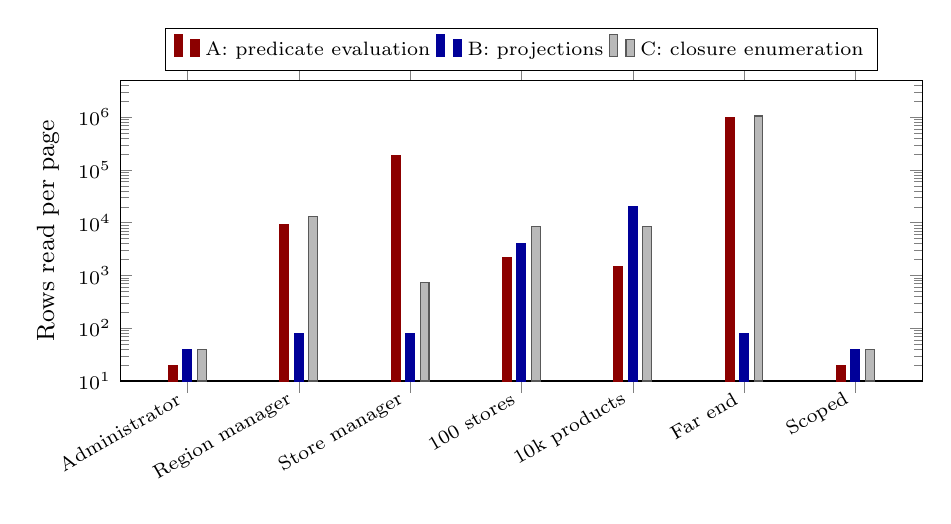
\begin{tikzpicture}
\begin{axis}[
    ybar, bar width=3.2pt, ymode=log, log origin=infty, ymin=10, ymax=5000000,
    symbolic x coords={Administrator,Region manager,Store manager,100 stores,10k products,Far end,Scoped},
    xtick=data, x tick label style={rotate=30, anchor=east, font=\scriptsize},
    ylabel={Rows read per page}, width=0.97\columnwidth, height=5.4cm,
    enlarge x limits=0.1, legend style={font=\scriptsize, at={(0.5,1.03)}, anchor=south, legend columns=3},
    every axis label/.style={font=\small}, every tick label/.style={font=\scriptsize},
]
\addplot[fill=red!55!black, draw=red!55!black] coordinates {(Administrator,20) (Region manager,9306) (Store manager,184205) (100 stores,2233) (10k products,1452) (Far end,980020) (Scoped,20)};
\addplot[fill=blue!60!black, draw=blue!60!black] coordinates {(Administrator,40) (Region manager,80) (Store manager,80) (100 stores,4040) (10k products,20040) (Far end,80) (Scoped,40)};
\addplot[fill=gray!55, draw=gray!70!black] coordinates {(Administrator,40) (Region manager,13263) (Store manager,742) (100 stores,8549) (10k products,8544) (Far end,1054147) (Scoped,40)};
\legend{A: predicate evaluation, B: projections, C: closure enumeration}
\end{axis}
\end{tikzpicture}
\caption{Rows read for the first page on PostgreSQL 16 by predicate evaluation (A), the proposed method (B) and closure enumeration (C), logarithmic scale.}
\label{fig:5}
\end{figure}



Under A, the rows read on PostgreSQL equal \(R\) (Table~\ref{tab:2}) and range from 20 to 980,020. For the store manager they fall from 184,205 to 80 on PostgreSQL and from 368,410 to 100 on SQL Server, and the time falls from 8,420 ms to 22.6 ms and from 179,558 ms to 89.0 ms. The region manager reads 80 rows under B instead of 9,306. The far-end caller, whose rows all occur at the end of the price order, reads 980,020 rows under A and 80 under B on PostgreSQL, and 1,960,040 and 100 on SQL Server; the time falls from 44,208 ms to 16.4 ms and from 942,593 ms to 90.3 ms. For every caller with one scope, B reads 80 rows on PostgreSQL: 20 in the scan phase, 40 in the merge phase (20 projection entries and the 20 rows on which \(\varphi\) is evaluated), and 20 in verification. SQL Server reads 100 because its scan phase reads each row twice. Under B, the position of the caller's rows in the order has no effect, since the range of the far-end caller's chain begins with its lowest-priced product.

\subsection{RQ2: Dense and Scoped Callers}\label{sec-7-4}

For the administrator, the time rises from 5.6 ms to 14.0 ms on PostgreSQL and from 23.7 ms to 52.3 ms on SQL Server, and the rows read from 20 to 40 on PostgreSQL. A executes one statement; B executes four, which resolve the caller's principals and the permission, scan 20 rows, and verify them. The scoped store manager shows the same pattern, at 5.4 ms against 12.8 ms on PostgreSQL and 18.4 ms against 39.4 ms on SQL Server. For both callers the scan phase completes the page, and B reads no projection.

\subsection{RQ3: Number of Granted Scopes}\label{sec-7-5}

The caller with grants on 100 stores reads 4,040 rows under B, 40 for each scope and 40 in the scan and verification phases, and takes 21.8 ms against 107.6 ms under A on PostgreSQL. The caller with 10,000 grants on individual products reads 20,040 rows under B on PostgreSQL, because each of its 10,000 scopes holds one product and the merge phase performs one range read per scope. A reads 1,452 rows for this caller, whose rows are distributed uniformly in price order, and takes 70.8 ms against 390.2 ms for B. On SQL Server the order of the times is reversed, at 1,420 ms for A and 762.7 ms for B, although B reads 20,060 rows against 2,904.

Table~\ref{tab:6} and Fig.~\ref{fig:6} report the callers with grants on 1 to 500 stores. The rows read by A fall as the caller's share of the table grows, from 193,501 to 367, in approximate proportion to \(P/\sigma\). The rows read by B are \(40 \cdot k + 40\) for \(k\) granted stores, from 80 to 20,040, and its time rises from 15.5 ms to 38.9 ms. Between 100 and 500 granted stores the order of the times reverses, and with 500 stores A takes 24.0 ms and B 38.9 ms. The cost of B is determined by the number of scopes and not by the share of the table; a caller with one grant on a higher-level scope, such as the region manager or the far-end caller, reads 80 rows whatever its share.

\begin{table*}[!tp]
\centering
\caption{Closure enumeration (C) on both engines, 1,000,000 products, first page of 20 rows ordered by price. The last column repeats the rows read by B from Tables~\ref{tab:3} and~\ref{tab:4}.}
\label{tab:5}
\scriptsize
\begin{adjustbox}{max width=\textwidth}
\begin{tabular}{@{}lrrrrrr@{}}
\toprule\noalign{}
Caller & \(\min(R, V)\) & C PostgreSQL: time (ms) & rows read & C SQL Server: time (ms) & rows read & B rows read (PostgreSQL / SQL Server) \\
\midrule\noalign{}
Administrator & 20 & 13.7 & 40 & 50.9 & 60 & 40 / 60 \\
Region manager & 2,000 & 951.3 & 13,263 & 2,644.3 & 19,364 & 80 / 100 \\
Store manager & 100 & 59.3 & 742 & 245.1 & 1,162 & 80 / 100 \\
100 stores & 2,233 & 875.2 & 8,549 & 2,701.8 & 15,364 & 4,040 / 4,060 \\
10,000 single products & 1,452 & 2,305.1 & 8,544 & 35,526.3 & 15,364 & 20,040 / 20,060 \\
Far end & 20,000 & 3,044.9 & 1,054,147 & 12,116.5 & 101,445 & 80 / 100 \\
Scoped store manager & 20 & 13.8 & 40 & 53.2 & 60 & 40 / 60 \\
\bottomrule
\end{tabular}
\end{adjustbox}
\end{table*}

\begin{table*}[!tp]
\centering
\caption{Selectivity sweep on PostgreSQL 16: callers with grants on \(k\) stores, first page of 20 rows ordered by price. A and C were measured in one run and B in a second run (Section~\ref{sec-7-2}).}
\label{tab:6}
\scriptsize
\begin{adjustbox}{max width=\textwidth}
\begin{tabular}{@{}rrrrrrrrrr@{}}
\toprule\noalign{}
Granted stores & \(V\) & Share & \(\min(R, V)\) & A: rows read & A: time (ms) & B: rows read & B: time (ms) & C: rows read & C: time (ms) \\
\midrule\noalign{}
1 & 100 & 0.01\% & 100 & 193,501 & 11,707.8 & 80 & 15.5 & 742 & 59.3 \\
10 & 1,000 & 0.1\% & 1,000 & 19,481 & 1,295.4 & 440 & 16.3 & 4,142 & 168.6 \\
45 & 4,500 & 0.45\% & 3,825 & 3,825 & 204.3 & 1,840 & 17.8 & 8,549 & 883.3 \\
100 & 10,000 & 1\% & 1,928 & 1,928 & 105.5 & 4,040 & 20.2 & 8,549 & 899.6 \\
500 & 50,000 & 5\% & 367 & 367 & 24.0 & 20,040 & 38.9 & 2,142 & 200.0 \\
\bottomrule
\end{tabular}
\end{adjustbox}
\end{table*}


\begin{figure}[!t]
\centering
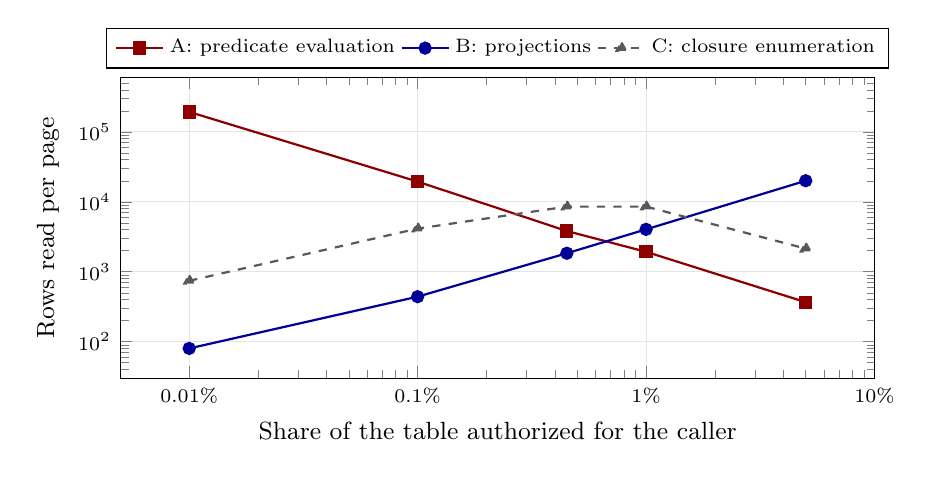
\begin{tikzpicture}
\begin{loglogaxis}[
    xlabel={Share of the table authorized for the caller}, ylabel={Rows read per page},
    width=0.92\columnwidth, height=5.4cm, grid=major, grid style={gray!20},
    ymin=30, ymax=600000,
    legend style={font=\scriptsize, at={(0.5,1.03)}, anchor=south, legend columns=3},
    every axis label/.style={font=\small}, every tick label/.style={font=\scriptsize},
    xtick={0.0001,0.001,0.01,0.1}, xticklabels={0.01\%,0.1\%,1\%,10\%}, xmax=0.1,
]
\addplot[color=red!55!black, thick, mark=square*] coordinates {(0.0001,193501) (0.001,19481) (0.0045,3825) (0.01,1928) (0.05,367)};
\addplot[color=blue!60!black, thick, mark=*] coordinates {(0.0001,80) (0.001,440) (0.0045,1840) (0.01,4040) (0.05,20040)};
\addplot[color=gray!70!black, thick, dashed, mark=triangle*] coordinates {(0.0001,742) (0.001,4142) (0.0045,8549) (0.01,8549) (0.05,2142)};
\legend{A: predicate evaluation, B: projections, C: closure enumeration}
\end{loglogaxis}
\end{tikzpicture}
\caption{Rows read for the first page on PostgreSQL 16 against the caller's share of the table, for callers with grants on 1 to 500 stores, logarithmic scales.}
\label{fig:6}
\end{figure}



\subsection{RQ4: Ordered Projections and Closure Enumeration}\label{sec-7-6}

Table~\ref{tab:5} reports C for the seven callers. On PostgreSQL, C reads between 2.0 and 7.4 times \(\min(R, V)\) rows for six of the seven callers, in 4 to 16 statements per page. For the far-end caller, C's fetch statement requested the caller's 20,000 rows by key; PostgreSQL's cost estimates for a parallel sequential scan of Products and for 20,000 primary-key lookups differed by 7\%, the optimizer selected the scan, and the page read 1,054,147 rows. With parallel query disabled, the same page read 74,145 rows in 2,603.1 ms. On SQL Server, C read 101,445 rows for this caller. For the caller with 10,000 single grants, C recomputes the caller's minimal scopes in each of its rounds; on SQL Server, the row limit of the closure statement propagated into the minimality computation, and one round took 25 s of the 35,526.3 ms.

For callers with one scope, B reads 80 rows on PostgreSQL where C reads 742 to 1,054,147, since C must read all of the caller's rows before it can order them, whereas B reads the first 20 entries of an ordered range. For the caller with 10,000 single grants, C reads fewer rows than B, 8,544 against 20,040, but takes 2,305.1 ms against 390.2 ms. In the selectivity sweep (Table~\ref{tab:6}), C reads fewer rows than A for the callers with 1 and 10 stores and more for the callers with 45, 100 and 500 stores, and more than B for every caller except the one with 500 stores. The ancestor closure removes the dependence of the cost on the position of the caller's rows, but not on their number, and the cost of reading the caller's rows by key depends on the access path that the optimizer selects. Ordering each scope's entries by the index key, as the projections do, removes both dependencies and leaves a dependence on the number of scopes.

\subsection{RQ5: Storage and Update Cost}\label{sec-7-7}

Table~\ref{tab:7} lists the projections of the Products table under version 11.0.0, which projects the primary key and both indexes. Each holds 6,000,000 entries, one per product and active ancestor, and occupies 550 MB to 866 MB. Writing all 18,000,000 entries with the rebuild procedure took 175 s on PostgreSQL. With version 10.0.0, building the price projection alone took 55 s on PostgreSQL and 200 s on SQL Server.

\begin{table}[!tp]
\centering
\caption{Projections of the Products table on PostgreSQL 16, 1,000,000 products with six active ancestors each.}
\label{tab:7}
\scriptsize
\begin{adjustbox}{max width=\columnwidth}
\begin{tabular}{@{}lrr@{}}
\toprule\noalign{}
Ordering & Entries & Size (MB) \\
\midrule\noalign{}
(Price, Id) & 6,000,000 & 706 \\
(StoreId, Price, Id) & 6,000,000 & 866 \\
(Id) & 6,000,000 & 550 \\
\bottomrule
\end{tabular}
\end{adjustbox}
\end{table}

Table~\ref{tab:8} compares write latency for an unprotected Products table and for the same table with three projections. Inserting one product with its resource writes six entries into each projection and takes 5.7 ms against 1.4 ms. Inserting 1,000 products in one save takes 635.6 ms against 211.8 ms. Moving a region of 2,000 products to another chain rewrites 12,000 entries in each projection and takes 501.0 ms against 5.2 ms. Both columns were measured with the two maintenance changes of Section~\ref{sec-6-3}.

\begin{table}[!tp]
\centering
\caption{Write latency on PostgreSQL 16 for an unprotected Products table and for the same table with three projections (median; 25 saves for the single insertion).}
\label{tab:8}
\scriptsize
\begin{adjustbox}{max width=\columnwidth}
\begin{tabular}{@{}lrr@{}}
\toprule\noalign{}
Operation & Unprotected (ms) & Three projections (ms) \\
\midrule\noalign{}
Insert one product & 1.4 & 5.7 \\
Insert 1,000 products in one save & 211.8 & 635.6 \\
Move a region of 2,000 products & 5.2 & 501.0 \\
\bottomrule
\end{tabular}
\end{adjustbox}
\end{table}

\subsection{Threats to Validity}\label{sec-7-8}

All measurements were taken on one laptop, with SQL Server under emulation, and times are medians of a small number of runs on a shared machine; the conclusions rest on the row counts, which are exact. The data is synthetic, with uniform prices, equal fan-out at every level and one resource per product, which gives every product the maximal ancestor path of the tree. Skew in the price distribution changes \(R\) but not the \(k \cdot P\) term of B. All measurements request the first page, and deep cursors were not measured, although the analysis of Section~\ref{sec-5} does not depend on the cursor. On PostgreSQL, statements were planned at every execution because the client did not prepare them. The measurements combine runs of two builds whose statements for A and B are identical, as the identical row counts confirm, and method C is not part of a released version. The correctness of B was checked by integration tests that compare every page with row-by-row point checks on both engines \cite{ref18}.

\section{Related Work}\label{sec-8}

\subsection{Enumeration in Authorization Services}\label{sec-8-1}

Zanzibar \cite{ref8} serves point checks at large scale and describes search as checking candidates, noting that search results ``often require tens to hundreds of checks''; clients that need other access paths maintain secondary indexes from its change stream, and its Leopard index precomputes flattened group membership. Services in the Zanzibar family answer enumeration by expanding the relationship graph backwards from the user. OpenFGA's ListObjects returns an unordered set bounded by a result limit and a deadline \cite{ref10}, and its maintainers state that it cannot be paginated because ``the graph evaluation is done concurrently (and thus is not ordered)'' \cite{ref22}. Auth0's documentation describes strategies that combine database queries, batch checks and list calls, and notes that a partial list ``is not enough, because you won't be able to sort using it'' \cite{ref23}. Materialization addresses ordering. AuthZed Materialize streams computed permissions into the application's database so that applications can ``sort, filter, and paginate over many thousands of authorized objects natively'' \cite{ref24}, and Auth0 FGA documents a precomputed permissions index \cite{ref23}. These systems materialize permission facts and update them asynchronously from a change stream. The projections of Section~\ref{sec-4} materialize structure, which changes with rows and resources but not with grants, and are updated in the writing transaction. Partitioning by scope also appears in search systems. Dropbox's search engine determines at query time the namespaces a user may read and retrieves documents within them \cite{ref25}, and Slack keeps a separate indexed copy of a message for each organization that shares a channel \cite{ref26}.

\subsection{Query Modification and Row-Level Security}\label{sec-8-2}

Query modification adds authorization predicates to queries \cite{ref27}, and row-level security in PostgreSQL and SQL Server builds it into the engine. PostgreSQL evaluates a policy expression for each row ``prior to any conditions or functions coming from the user's query'' \cite{ref28}. Supabase's guidance states that the cost scales with the rows a query scans and recommends indexing the columns that policies filter on and evaluating functions once per statement \cite{ref29}. Microsoft's guidance for SQL Server row-level security is to avoid recursion in predicate functions \cite{ref30}, and practitioners recommend flattening hierarchies before they are used in predicates \cite{ref31}. Policy engines compile policies into query conditions. Oso generates SQL filters \cite{ref32}, Cerbos returns a condition tree for translation into a query \cite{ref33}, and Open Policy Agent derives filters by partial evaluation \cite{ref34}. When the authorized set cannot be expressed as a condition on an indexed column of the table, as with grants at arbitrary levels of a hierarchy, the database evaluates such predicates on rows in the order in which the query reads them, and the cost of ordered pagination follows \(R\) as in Section~\ref{sec-3-2}.

\subsection{Hierarchy Encodings and Merging}\label{sec-8-3}

Closure tables store one row per ancestor--descendant pair, which makes subtree queries simple and makes moves rewrite the pairs of the moved subtree \cite{ref35}. The hierarchyid type of SQL Server orders nodes depth-first, so that a depth-first index places every subtree contiguously \cite{ref36}; Spanner's interleaved tables store child rows under their parent's key \cite{ref37}; and nested intervals encode containment in numeric intervals \cite{ref38}. Each encoding provides one order per subtree, the order of the hierarchy itself. A projection of Section~\ref{sec-4} is a closure table extended with the key of an index, maintained once for every projected ordering. The merge phase of Algorithm~\ref{alg:1} is a \(k\)-way merge of sorted ranges. The threshold algorithm of Fagin et al.~\cite{ref39} addresses the more general problem of combining scores from several sorted lists; Algorithm~\ref{alg:1} requires only a merge because each authorized row occurs in exactly one range.

\section{Limitations and Future Work}\label{sec-9}

Storage and write cost grow with the number of projected orderings and the depth of the hierarchy. With three projected orderings and six active ancestors, each product has eighteen projection entries, which every insertion writes. Indexes created for filtering, such as (StoreId, Price, Id), are projected as well; that projection occupies 866 MB in Table~\ref{tab:7}, although no measured query orders by it, and the implementation provides no per-index exclusion. Moving a resource rewrites the entries of every row below it.

Sort columns must be non-nullable, because they form part of the projection's primary key, and an ordering on a nullable column is served by the scan phase alone. A caller with many individual grants pays one range read per scope (Section~\ref{sec-5-5}). A permission restricted to a resource type that some rows below a caller's scopes do not have can produce pages with fewer than \(P\) rows (Section~\ref{sec-5-2}). In a hierarchy of entity types mapped to one table, only the indexes of the root type are projected.

The implementation maintains projections in the application's database context. Writes that bypass it, such as bulk loads and raw SQL statements, leave projections inconsistent until a rebuild. Under snapshot isolation, a save that moves or deactivates a resource and a concurrent save that changes rows below it can leave those rows' entries on the old path, and under locking isolation either save can fail with a deadlock or a duplicate key. Rows with stale entries can be missing from pages until a rebuild, and verification prevents stale entries from exposing rows; the implementation does not take a lock that every save would contend on.

Several extensions follow from these limitations. Maintaining projections inside the database engine, through statement-level triggers or an extension, would keep them consistent for every writer; Definition 3 and the rebuild procedure specify the required result. A SQL function that returns an authorized page would make the method available to clients that do not use the library. Encoding nulls as ordered key values would allow nullable sort columns. Omitting the row lookups of the merge phase when \(Q\) has no filter would remove half of the rows that phase reads. Measurements on native SQL Server hardware, larger tables, skewed distributions and deep cursors would complement the evaluation of Section~\ref{sec-7}.

\section{Conclusion}\label{sec-10}

Scoped hierarchical role-based access control makes individual authorization decisions inexpensive but leaves ordered enumeration of authorized rows dependent on where those rows occur in the sort order. With predicate evaluation in index order, the rows examined per page are the rows that precede the \(P\)-th authorized row; with enumeration through an unordered ancestor closure, they are the caller's authorized rows. Ancestor-partitioned index projections order the rows below every scope by each index of a protected table. A page then requires the first \(P\) entries of each of the caller's \(k\) minimal scopes and costs \(O(P \cdot D \cdot M \cdot G_{\max} + G \cdot D + k \cdot P \log k)\), independent of the table size and of the caller's selectivity, while soundness rests on the unchanged access predicate. In experiments with 1,000,000 rows on two engines, pages for callers with one scope read 80 to 100 rows wherever their rows occur in the order. The cost is one projection entry per row and active ancestor for each projected ordering, and the corresponding work on every write.

\section*{AI Disclosure}

In accordance with IEEE policy, the author discloses that AI tools (Claude, Anthropic) were used to assist with manuscript preparation and editing and with the implementation and benchmarking work described. The technical decisions and the experimental design are the work of the author.

\balance

\begin{thebibliography}{39}
\bibitem{ref1} R. Sandhu, E. J. Coyne, H. L. Feinstein, and C. E. Youman, ``Role-Based Access Control Models,'' \emph{IEEE Computer}, vol. 29, no. 2, pp. 38--47, 1996.
\bibitem{ref2} D. F. Ferraiolo, R. Sandhu, S. Gavrila, D. R. Kuhn, and R. Chandramouli, ``Proposed NIST Standard for Role-Based Access Control,'' \emph{ACM Trans. Information and System Security}, vol. 4, no. 3, pp. 224--274, 2001.
\bibitem{ref3} Microsoft, ``What is Azure role-based access control (Azure RBAC)?,'' Microsoft Learn. \url{https://learn.microsoft.com/en-us/azure/role-based-access-control/overview} (accessed Oct. 2026).
\bibitem{ref4} Microsoft, ``Understand Azure role assignments,'' Microsoft Learn. \url{https://learn.microsoft.com/en-us/azure/role-based-access-control/role-assignments} (accessed Oct. 2026).
\bibitem{ref5} Microsoft, ``Understand scope for Azure RBAC,'' Microsoft Learn. \url{https://learn.microsoft.com/en-us/azure/role-based-access-control/scope-overview} (accessed Oct. 2026).
\bibitem{ref6} WorkOS, ``Fine-Grained Authorization (FGA),'' WorkOS Documentation. \url{https://workos.com/docs/fga/index} (accessed Oct. 2026).
\bibitem{ref7} OpenFGA, ``Parent-Child Objects,'' OpenFGA Documentation. \url{https://openfga.dev/docs/modeling/parent-child} (accessed Oct. 2026).
\bibitem{ref8} R. Pang, R. Caceres, M. Burrows, Z. Chen, P. Dave, N. Germer, A. Golynski, K. Graney, N. Kang, L. Kissner, J. L. Korn, A. Parmar, C. D. Richards, and M. Wang, ``Zanzibar: Google's Consistent, Global Authorization System,'' in \emph{Proc. USENIX ATC}, pp. 33--46, 2019.
\bibitem{ref9} R. Slaney, ``Database-Native Authorization for Human and Autonomous Principals: The SHRBAC Model,'' in \emph{Proc. IEEE COMPSAC}, 2026.
\bibitem{ref10} OpenFGA, ``Configuration,'' OpenFGA Documentation (listObjectsDeadline, listObjectsMaxResults). \url{https://openfga.dev/docs/getting-started/setup-openfga/configuration} (accessed Oct. 2026).
\bibitem{ref11} AuthZed, ``Protecting a list endpoint,'' SpiceDB Documentation. \url{https://authzed.com/docs/spicedb/modeling/protecting-a-list-endpoint} (accessed Oct. 2026).
\bibitem{ref12} Z. Zhang, X. Zhang, and R. Sandhu, ``ROBAC: Scalable Role and Organization Based Access Control Models,'' in \emph{Proc. CollaborateCom}, 2006.
\bibitem{ref13} N. Solanki et al., ``Resource and Role Hierarchy Based Access Control for Resourceful Systems,'' in \emph{Proc. IEEE COMPSAC}, pp. 396--401, 2018.
\bibitem{ref14} Microsoft, ``Understand Azure role definitions,'' Microsoft Learn. \url{https://learn.microsoft.com/en-us/azure/role-based-access-control/role-definitions} (accessed Oct. 2026).
\bibitem{ref15} Microsoft, ``Organize your resources with management groups,'' Microsoft Learn. \url{https://learn.microsoft.com/en-us/azure/governance/management-groups/overview} (accessed Oct. 2026).
\bibitem{ref16} Microsoft, ``List Azure deny assignments,'' Microsoft Learn. \url{https://learn.microsoft.com/en-us/azure/role-based-access-control/deny-assignments} (accessed Oct. 2026).
\bibitem{ref17} Microsoft, ``What is Privileged Identity Management?,'' Microsoft Learn. \url{https://learn.microsoft.com/en-us/entra/id-governance/privileged-identity-management/pim-configure} (accessed Oct. 2026).
\bibitem{ref18} R. Slaney, ``SqlOS,'' open-source library (MIT license), version 11.0.0, Oct. 2026. \url{https://github.com/ross-slaney/sqlos}
\bibitem{ref19} R. Slaney, benchmark results for SqlOS 10.0.0 on SQL Server 2022 and PostgreSQL 16, ross-slaney/sqlos pull request 516, Oct. 2026. \url{https://github.com/ross-slaney/sqlos/pull/516}
\bibitem{ref20} R. Slaney, benchmark results for SqlOS 11.0.0 on PostgreSQL 16, ross-slaney/sqlos pull request 524, Oct. 2026. \url{https://github.com/ross-slaney/sqlos/pull/524}
\bibitem{ref21} R. Slaney, benchmark results for closure enumeration and the selectivity sweep, ross-slaney/sqlos pull request 522, Oct. 2026. \url{https://github.com/ross-slaney/sqlos/pull/522}
\bibitem{ref22} OpenFGA maintainers, reply on ListObjects pagination, OpenFGA GitHub discussion 105, Jan. 2023. \url{https://github.com/orgs/openfga/discussions/105}
\bibitem{ref23} Auth0, ``Search with permissions,'' Auth0 FGA Documentation. \url{https://docs.fga.dev/integration/advanced/search-with-permissions} (accessed Oct. 2026).
\bibitem{ref24} AuthZed, ``AuthZed Materialize,'' AuthZed Documentation. \url{https://authzed.com/docs/authzed/concepts/authzed-materialize} (accessed Oct. 2026).
\bibitem{ref25} Dropbox, ``Architecture of Nautilus, the new Dropbox search engine,'' Dropbox Tech Blog, Sept. 2018. \url{https://dropbox.tech/machine-learning/architecture-of-nautilus-the-new-dropbox-search-engine}
\bibitem{ref26} Slack, ``Slack search powers visibility and compliance across your organisation,'' Slack Blog. \url{https://slack.com/blog/developers/enterprise-ai-search-with-slack-search}
\bibitem{ref27} M. Stonebraker and E. Wong, ``Access Control in a Relational Data Base Management System by Query Modification,'' in \emph{Proc. ACM Annual Conf.}, pp. 180--187, 1974.
\bibitem{ref28} PostgreSQL Global Development Group, ``Row Security Policies,'' PostgreSQL Documentation. \url{https://www.postgresql.org/docs/current/ddl-rowsecurity.html}
\bibitem{ref29} Supabase, ``Row Level Security performance,'' Supabase Documentation. \url{https://supabase.com/docs/guides/database/postgres/row-level-security-performance}
\bibitem{ref30} Microsoft, ``Row-Level Security,'' SQL Server Documentation. \url{https://learn.microsoft.com/en-us/sql/relational-databases/security/row-level-security}
\bibitem{ref31} B. Johnston, ``SQL Server RLS performance and troubleshooting,'' Redgate Simple Talk, Sept. 2023. \url{https://www.red-gate.com/simple-talk/databases/sql-server/sql-server-rls-performance-and-troubleshooting/}
\bibitem{ref32} Oso, ``Local Authorization,'' Oso Documentation. \url{https://www.osohq.com/docs/develop/facts/local-authorization}
\bibitem{ref33} Cerbos, ``Filtering resources by permission,'' Cerbos Documentation. \url{https://docs.cerbos.dev/cerbos/latest/recipes/filtering-resources}
\bibitem{ref34} Open Policy Agent, ``Data Filtering,'' OPA Documentation. \url{https://www.openpolicyagent.org/docs/filtering/}
\bibitem{ref35} B. Karwin, ``Moving Subtrees in Closure Table Hierarchies,'' Percona Blog, Feb. 2011. \url{https://www.percona.com/blog/moving-subtrees-in-closure-table/}
\bibitem{ref36} Microsoft, ``Hierarchical Data (SQL Server),'' SQL Server Documentation. \url{https://learn.microsoft.com/en-us/sql/relational-databases/hierarchical-data-sql-server}
\bibitem{ref37} Google Cloud, ``Schemas overview,'' Spanner Documentation. \url{https://docs.cloud.google.com/spanner/docs/schema-and-data-model}
\bibitem{ref38} V. Tropashko, ``Nested Intervals Tree Encoding in SQL,'' arXiv:cs/0402051, 2004.
\bibitem{ref39} R. Fagin, A. Lotem, and M. Naor, ``Optimal Aggregation Algorithms for Middleware,'' \emph{J. Computer and System Sciences}, vol. 66, no. 4, pp. 614--656, 2003.
\end{thebibliography}

\end{document}
